\documentclass[10pt]{beamer}

\mode<presentation>
{
  \usetheme[height=1.25cm]{Madrid}
  \setbeamertemplate{navigation symbols}{}
  \setbeamercolor{alerted text}{fg=illini}
}
\usebackgroundtemplate{
\includegraphics[width=\paperwidth,height=\paperheight]{uc-background}}

\usepackage[english]{babel}
\usepackage{epsfig,subfigure,bm}
\usepackage{multimedia}
\usepackage{psfrag}
\usepackage{animate}

%%%%%% Begin of my macros and options

\setbeamertemplate{section in toc shaded}[default][55]
\setbeamertemplate{subsection in toc shaded}[default][55]
\setbeamercolor{block title}{fg=white,bg=illini}
\setbeamercolor{block body}{fg=black,bg=mygrey}

\setbeamercolor{emphprimary}{fg=CBlue}
\setbeamercolor{emphsecondary}{fg=illini}
\setbeamercolor{emphtertiary}{fg=mygreen}
\definecolor{darkForestGreen}{rgb}{.1,1,.1}
\definecolor{veryLightGray}{rgb}{.9,.9,.9}
\definecolor{greenApple}{rgb}{.3,.9,.3}

\setbeamercolor{frametitle}{bg=CBlue}   
\setbeamercolor{title}{bg=CBlue}

\usepackage{amsmath,amssymb,amsxtra,amsthm,mathlib_4}
\usepackage{algorithm,algorithmic}
\usepackage{natbib}
\usepackage{bibentry}
\usepackage{xspace}
\usepackage{changepage}

\pdfmapfile{+sansmathaccent.map}

\definecolor{myblue}{rgb}{.2,.2,.7}
\definecolor{myred}{rgb}{.7,.2,.2}
\definecolor{mygreen}{rgb}{.2,.7,.2}
\definecolor{mygrey}{rgb}{0.9,0.9,0.9}
\definecolor{CBlue}{cmyk}{1,0.25,0,0}
\definecolor{illini}{rgb}{0.98,0.4,0.05}
\definecolor{black}{cmyk}{0,0,0,1}

\newcommand{\myemph}[1]{{\usebeamercolor[fg]{emphprimary}
    \textbf{#1}}}
\newcommand{\myemphalt}[1]{{\usebeamercolor[fg]{emphsecondary}
    \textbf{#1}}}

\graphicspath{{figs/}}

\title[MURO Lab] % (optional, use only with long paper titles)
{Multi-Agent Robotics (MURO) Lab}

\author[J. Cort\'es, S. Mart{\'\i}nez] % (optional, use only with lots of authors)
{Jorge Cort\'es and Sonia Mart{\'\i}nez}
% - Give the names in the same order as the appear in the paper.  -
% Use the \inst{?} command only if the authors have different
% affiliation.

\institute[UCSD] % (optional, but mostly needed)
{
  \begin{minipage}[c]{.2\textwidth}
    \includegraphics[width=.65\linewidth]{ucsealnew}%
  \end{minipage}%
  \begin{minipage}[c]{.6\textwidth}
    \small 
    Mechanical and Aerospace Engineering\\
    University of California, San Diego\\
    \myemph{\url{http://muro.ucsd.edu}}\\
  \end{minipage}
%%  \vspace*{1ex}
}
%% - Use the \inst command only if there are several affiliations.
%% - Keep it simple, no one is interested in your street address.

\bigskip

\date[February 26,
2018]% (optional, should be abbreviation of conference name)
{\small%
  Unmanned Logistics Systems
  \\
  UC San Diego
  \\
  February 26, 2018}

\begin{document}
  
\nobibliography{alias,JC,Main,New}
\bibliographystyle{plain}

\begin{frame}[plain]
  \titlepage
\end{frame}

\begin{frame}
  \frametitle{MURO Lab for Swarm Robotics}
  
\vspace*{-0.8cm}


\hspace*{7.5cm}\begin{minipage}[r]{0.40\linewidth}
  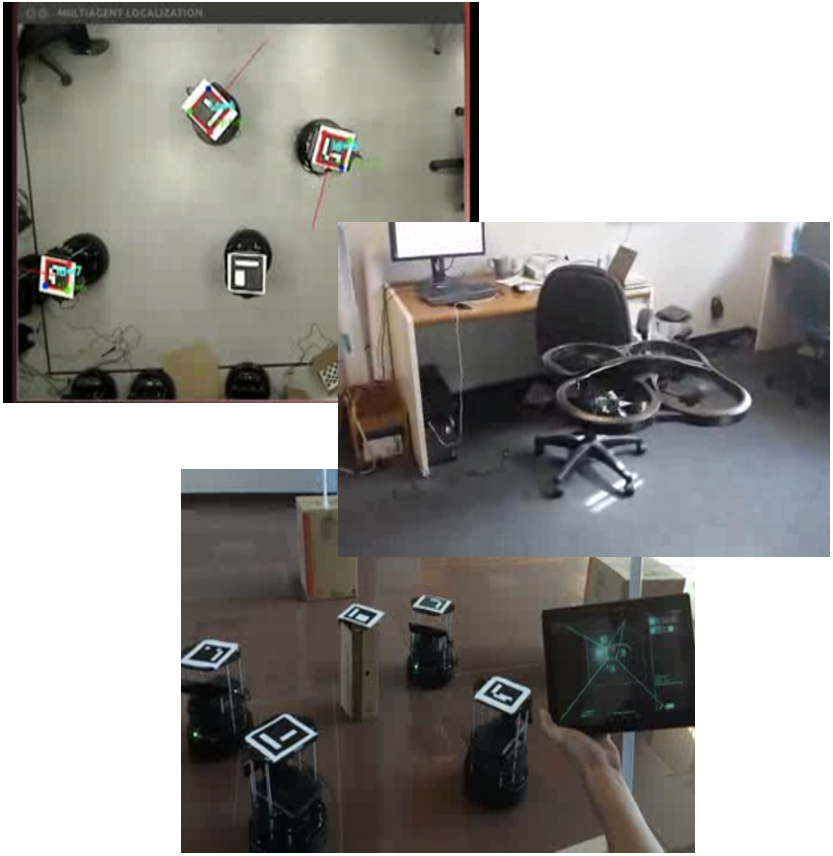
\includegraphics[height=.9\linewidth]{lab-pics}
\end{minipage}

\vspace*{-4.5cm}

\myemph{Analysis and design tools} to develop  \\
\hspace*{0.5cm} provably correct algorithms \\
\hspace*{0.5cm} Demonstrated on simulation \\
\hspace*{0.5cm} and robotic  testbeds

\vspace*{0.3cm}

\myemph{Models} to formalize, analyze and \\
\hspace*{0.5cm}compare coordination algorithms\\
\hspace*{0.5cm}useful in sensing, estimation, planning
 
\vspace*{0.3cm} 

\myemph{Example problems:} formation control, coverage 
\\\hspace*{0.5cm}control, task assignment, distributed
estimation

\bigskip

    \begin{center}
        \setlength{\tabcolsep}{2pt}
  \begin{tabular}{cccc}
    \href{run:animations/run-RangeBased-area-addition-animation.mov}%
    {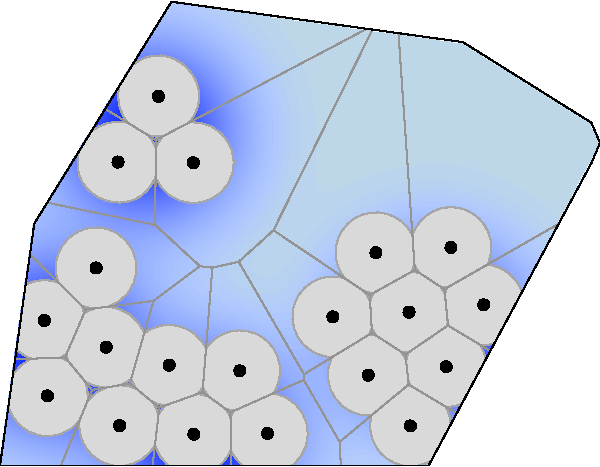
\includegraphics[width=.2\linewidth]{run-RangeBased-area-final}}
    &
    \href{run:animations/artgallery-partition+centering+heuristic-19feb04.mov}
    {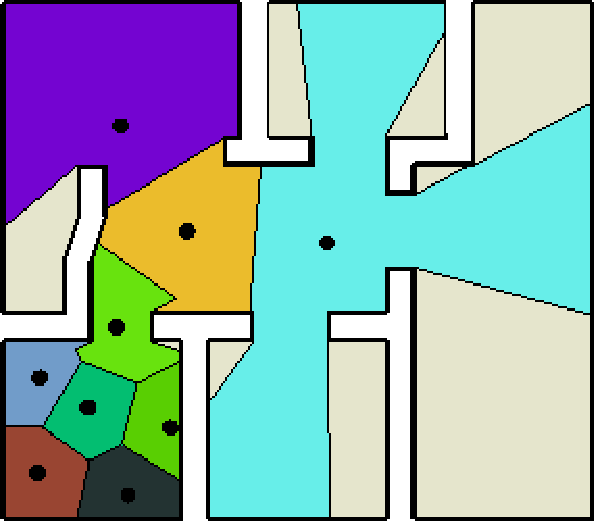
\includegraphics[width=.18\linewidth]{artgallery-partition+centering+heuristic-19feb04-midway}}
    \href{run:lab/gaussian_normal_moving.mov}{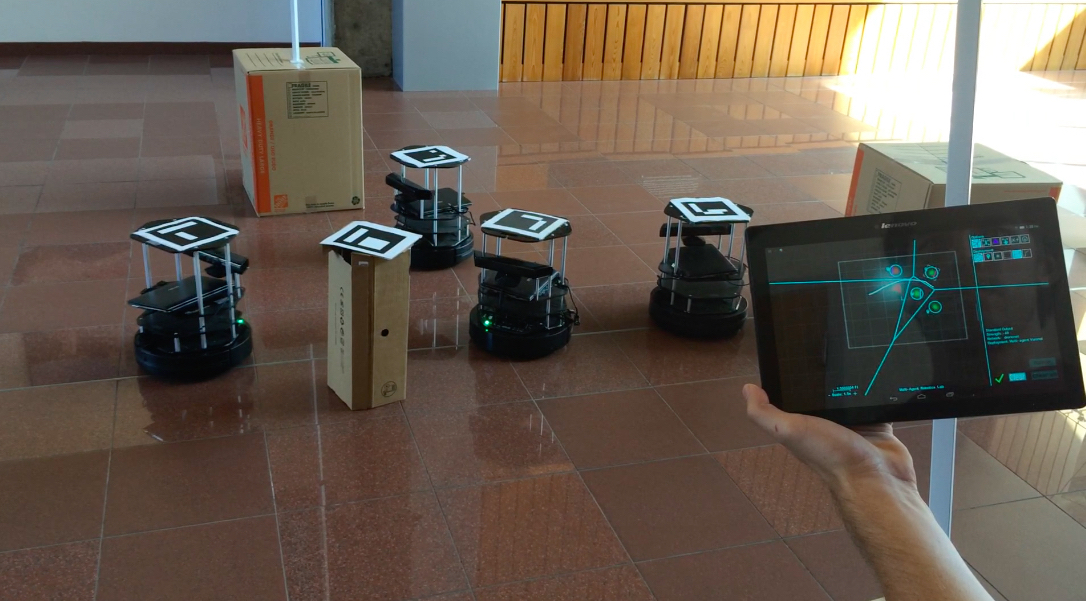
\includegraphics[width=.22\linewidth]{deployment-lobby-EBUI}}
    &
    \href{run:movies/toward-circumcenter-3D-animation.mov}%
    {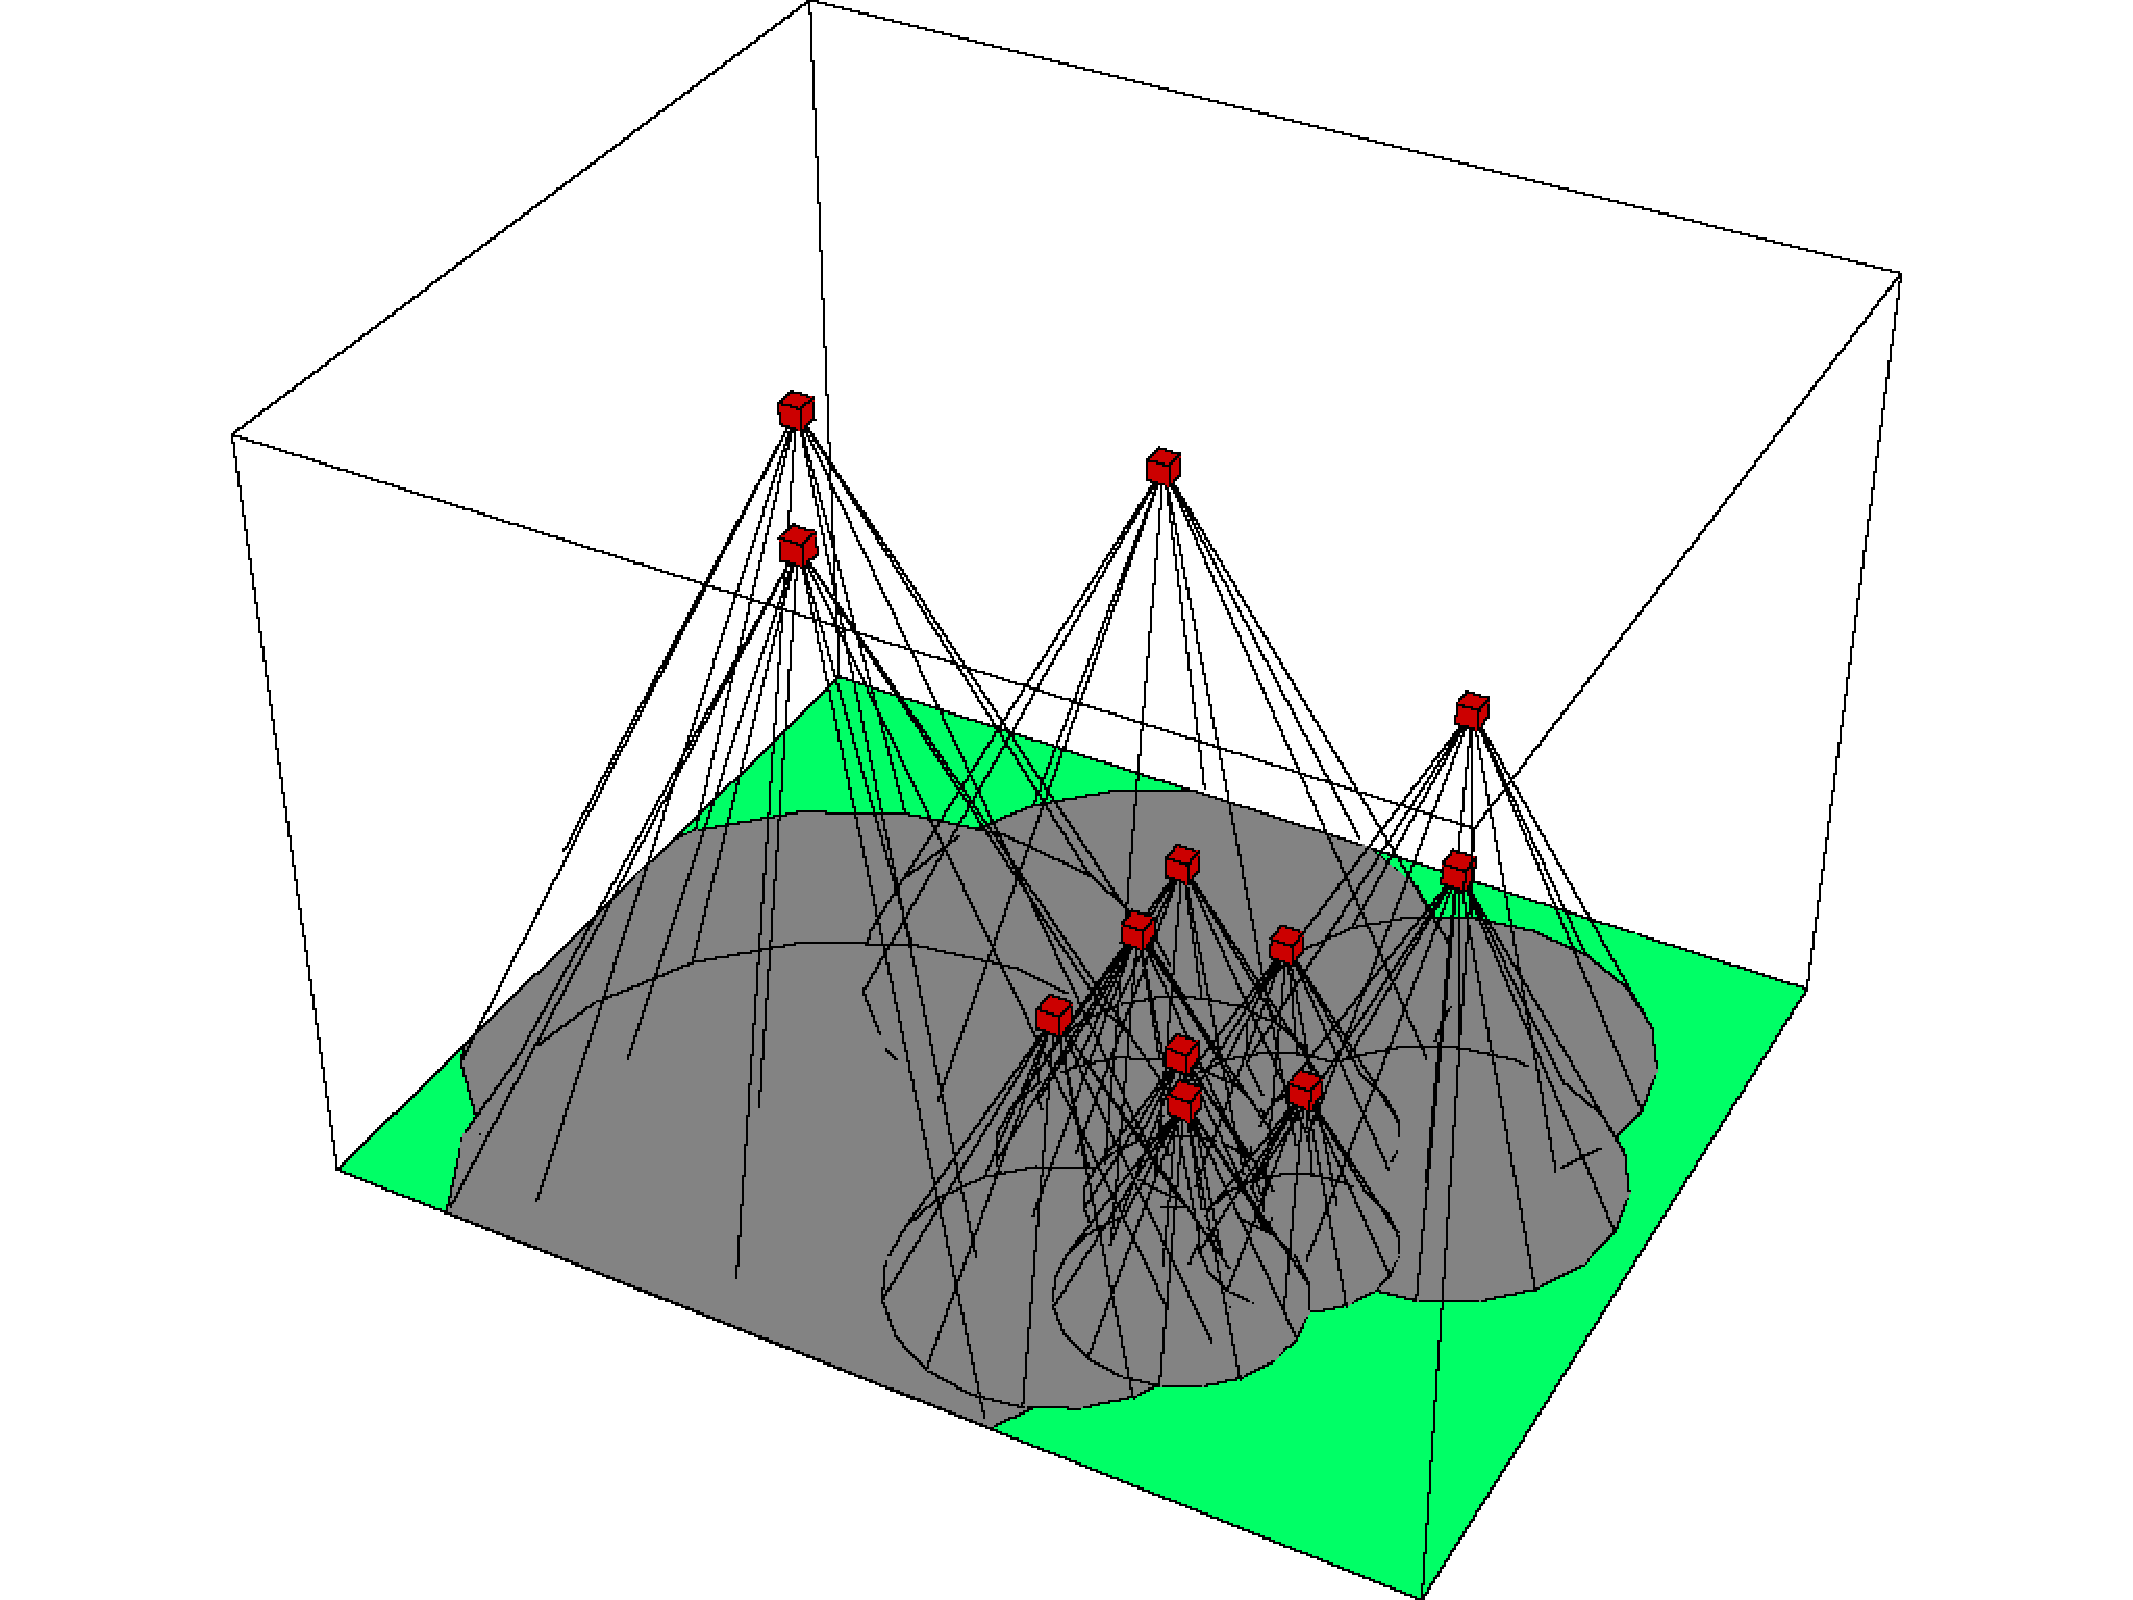
\includegraphics[width=.22\linewidth]{3d-coverage}}%    
    \\[-1ex]
    \tiny{Limited-range} &
    \tiny{Distributed art gallery} &
    \tiny{Human-swarm interaction} &    
    \tiny{3D deployment}
  \end{tabular}
    \end{center}

\vspace*{-2cm}


\end{frame}

\begin{frame}

  \frametitle{Disaster Response and Recovery}
  \framesubtitle{Northrop Grumman (M. Milam, R. Chen)--UCSD (K. Lee,
    S. Martinez, JC) collaboration}

  \begin{center}
    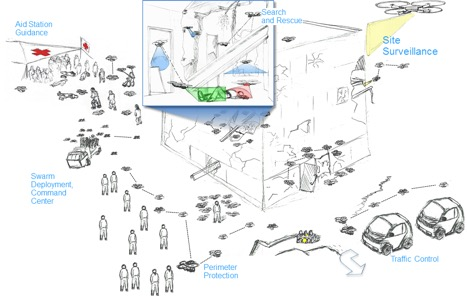
\includegraphics[width=.65\linewidth]{swarm-disaster-response}
  \end{center}

  {\small \myemph{Multi-robot control} for
    \\[.5ex]
  \begin{tabular}{ll}
  assess scope and severity of disaster
  &
  search and rescue
  \\
  maintain safety perimeter
  &
  reroute traffic
  \\
  provide situational awareness
  & 
  suggest paths for emergency responders
  \end{tabular}
}  
  
\end{frame}

\begin{frame}

  \frametitle{Underwater Mine Detection}
  \framesubtitle{Spawar (M. Ouimet, V. Djapic)--UCSD (A. Ma,
    S. Martinez, JC) collaboration}

  \begin{center}
  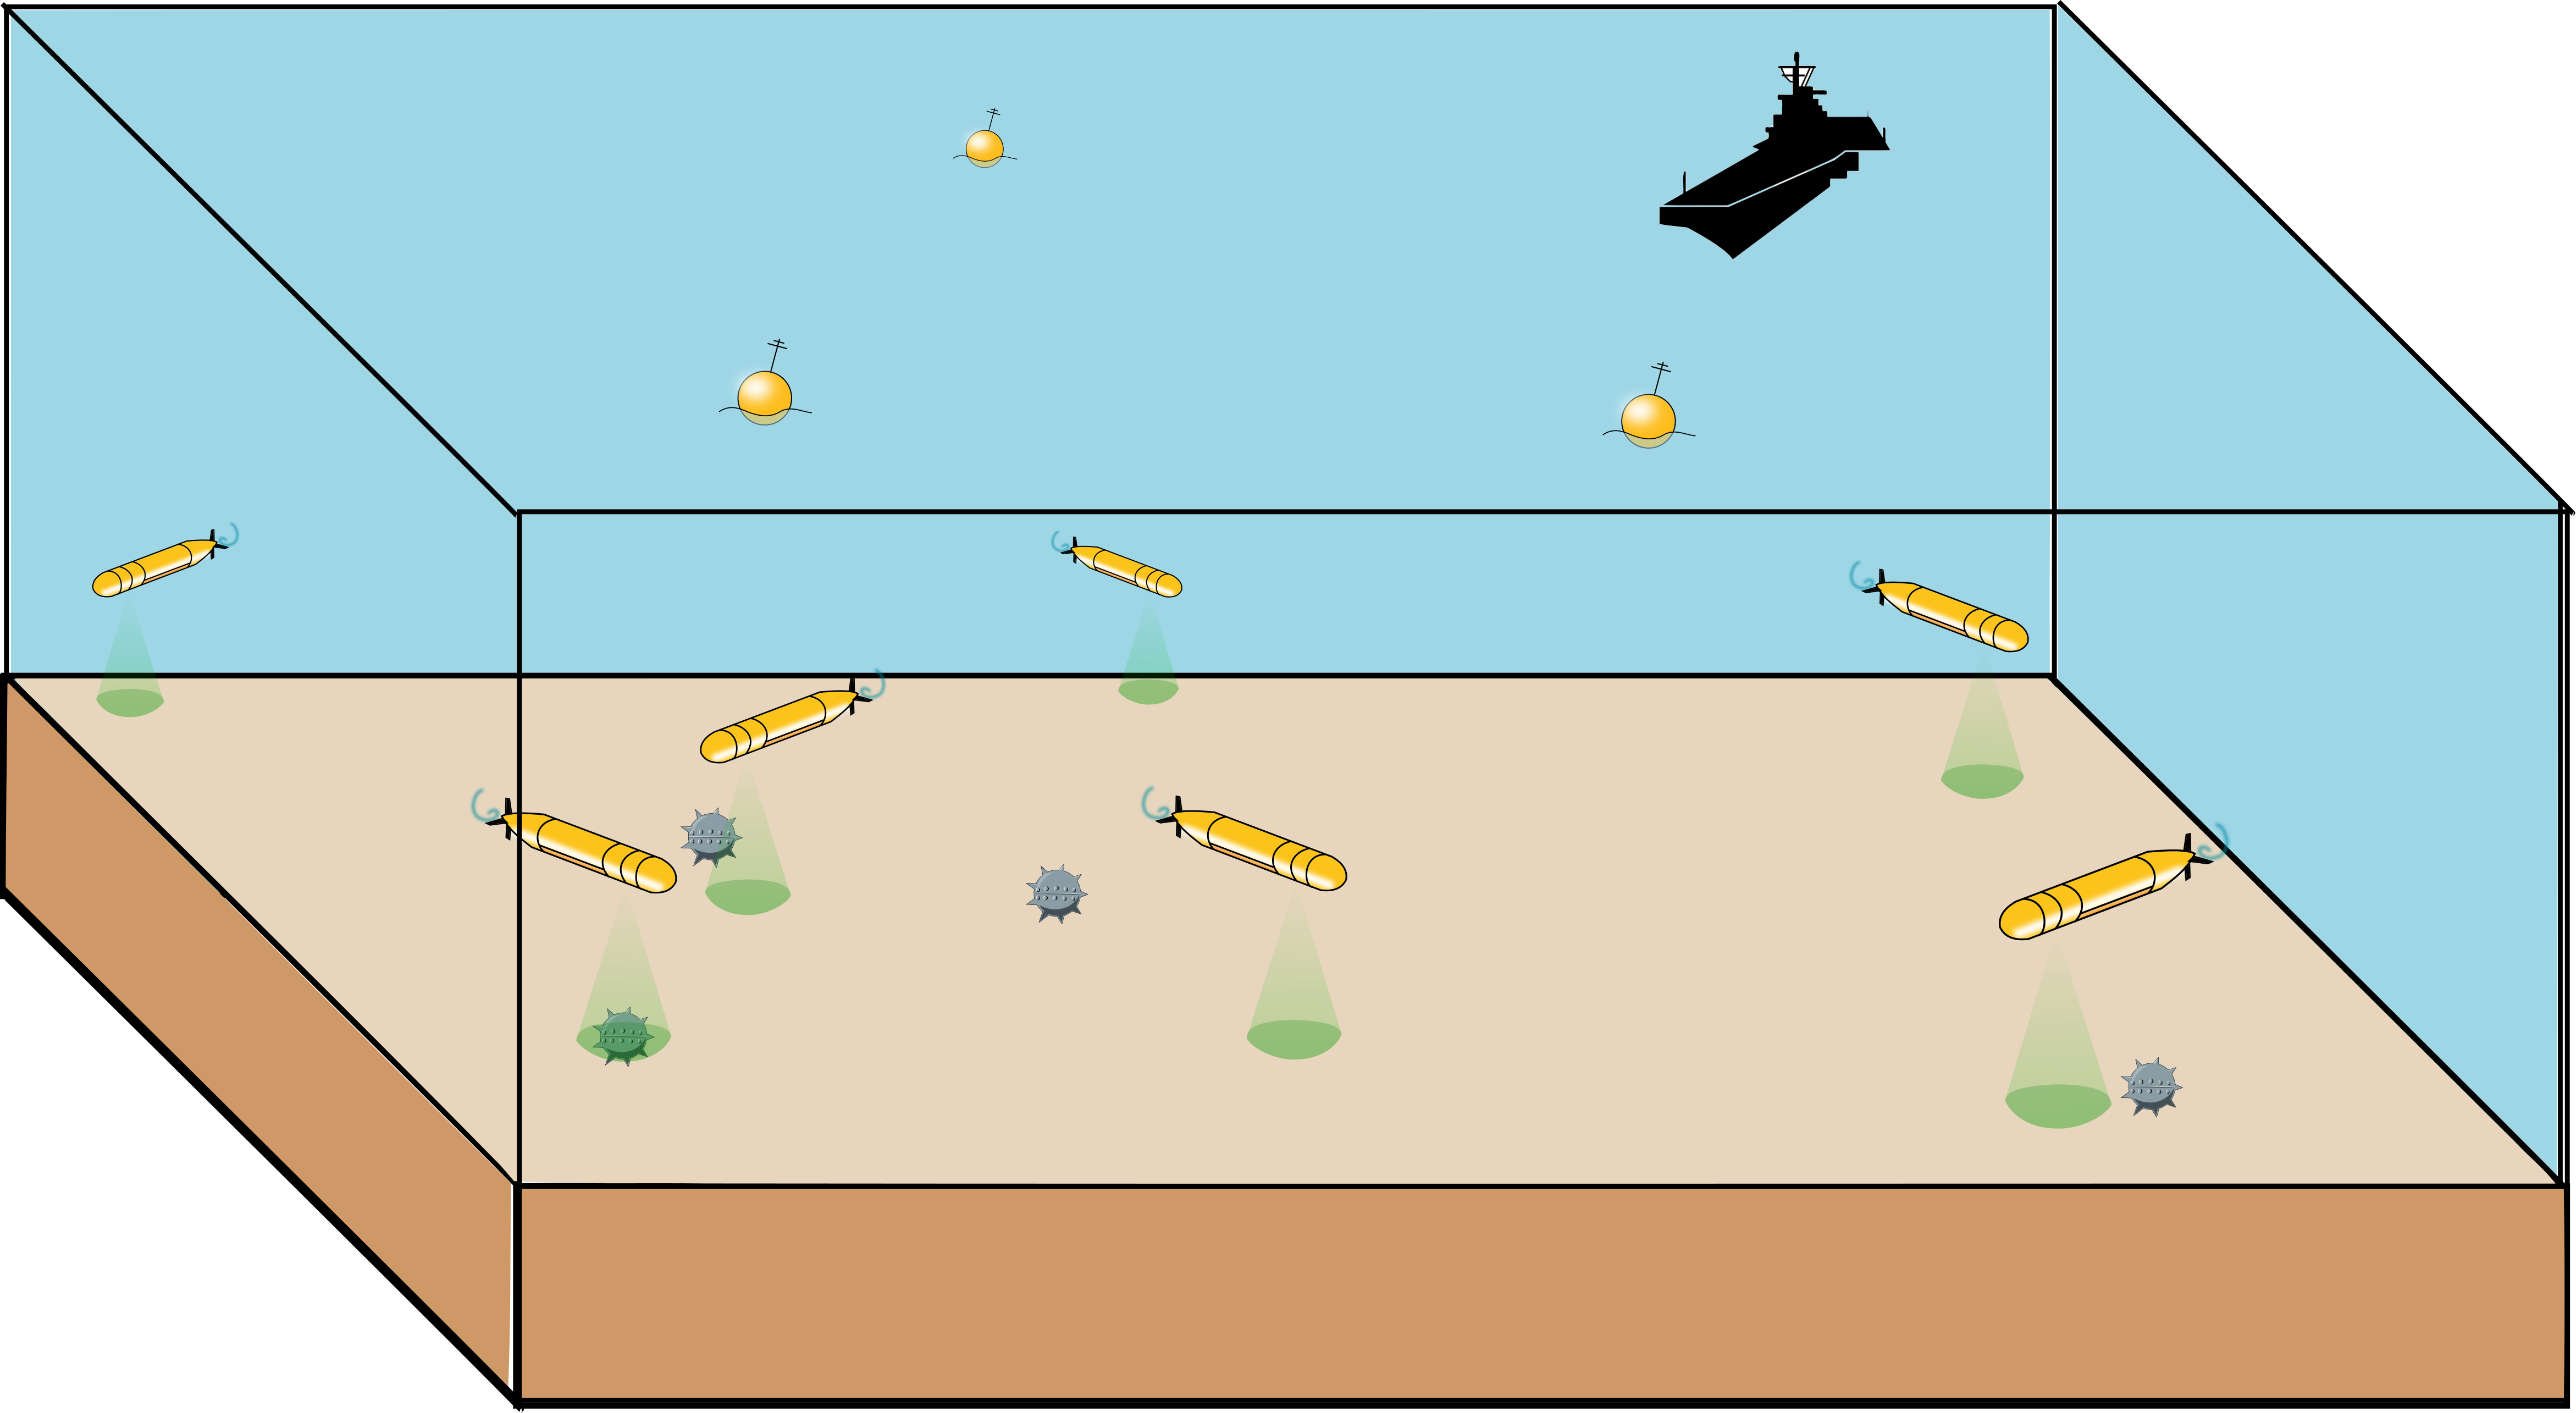
\includegraphics[width=.65\linewidth]{swarm-mines-detection}
  \end{center}

  {\small \myemph{Multi-robot control} for
    \\[.5ex]
  \begin{tabular}{ll}
    detect mines
    &
    service mines
    \\
    re-charge
    &
    act as relays for inter-robot communication
    \\
    provide situational awareness
    & 
    support for localization
  \end{tabular}
}  
  
\end{frame}


\begin{frame}

  \frametitle{Shared Autonomy: Human-Swarm Coordination}

    \alert{Abstractions} enabling swarm control by human operator with
    guaranteed behavior
    \begin{itemize}
    \item how to relay human intent to swarm?
    \item how can swarm recognize human intent?
    \end{itemize}
    
    \begin{center}
      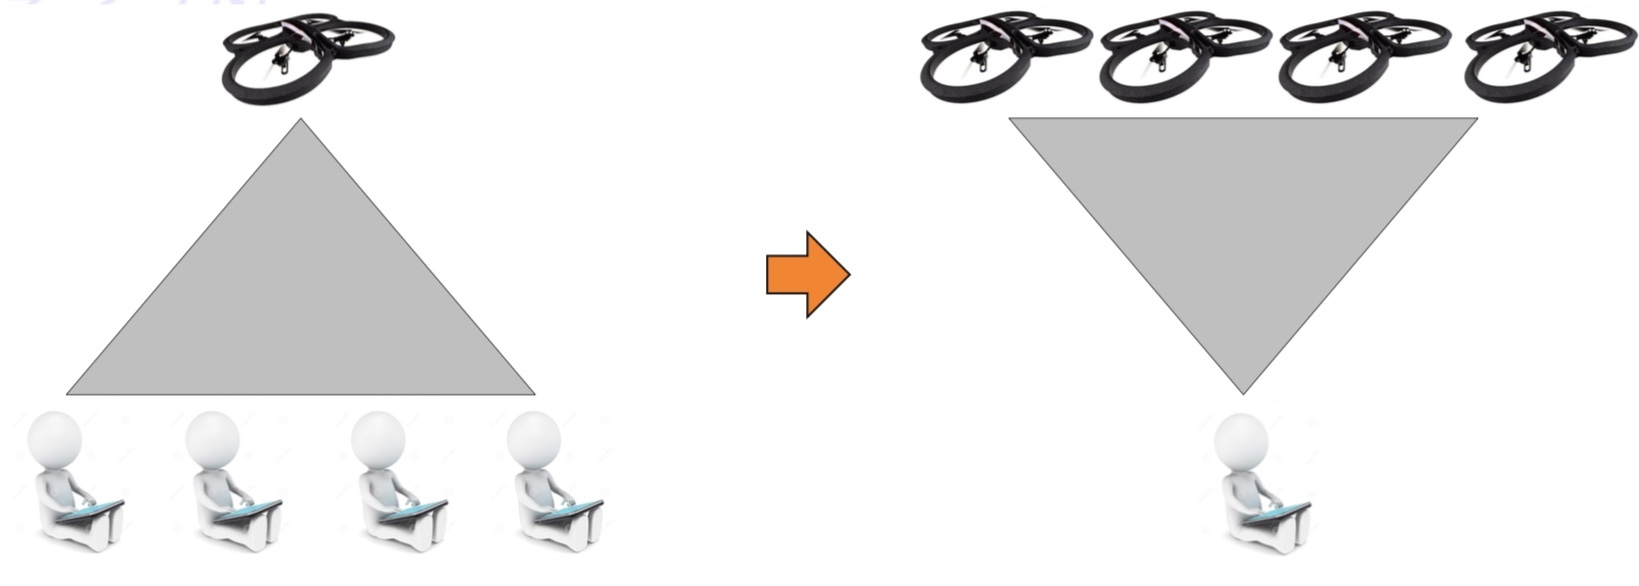
\includegraphics[width=.7\linewidth]{human-swarm}      
    \end{center}

  \onslide<2>{
  Focus on \alert{`systems'} questions

  \medskip
  \begin{minipage}{.9\linewidth}
    \begin{itemize}
    \item predictability of swarm behavior disturbed by human input?
    \item how to make swarm easy/difficult to control?
    \item robustness, speed of convergence, interconnection
    \end{itemize}    
  \end{minipage}
}

\end{frame}

\begin{frame}
  \frametitle{Human-Swarm Optimal Deployment}

  \begin{overprint}
    \onslide<1>

  \begin{minipage}{.625\linewidth}
    \alert{Human} specifies importance function\newline \null \mbox{}
    \hfill \phantom{-- through tablet app}

    \bigskip
    
    \alert{Robot swarm} deploys according to specification

    \bigskip

    Changes in function induce swarm reconfiguration
  \end{minipage}
  \hfill
  \begin{minipage}{.315\linewidth}
    {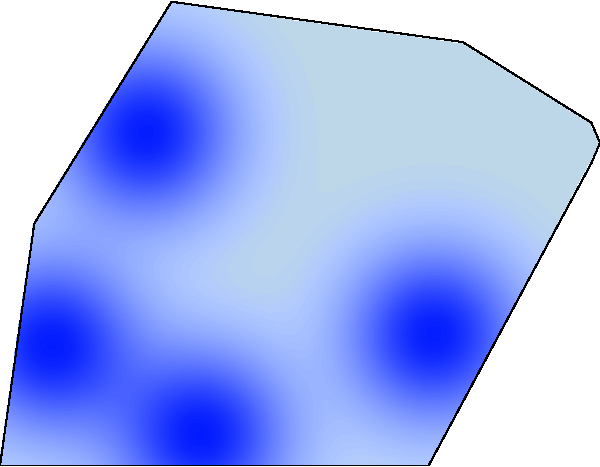
\includegraphics[width=.775\linewidth]{phicontourplot-nicest}}
  \end{minipage}

    \onslide<2>

  \begin{minipage}{.625\linewidth}
    \alert{Human} specifies importance function\newline
    \null \mbox{} \hfill -- through tablet app

    \bigskip
    
    \alert{Robot swarm} deploys according to specification

    \bigskip

    Changes in function induce swarm reconfiguration
  \end{minipage}
  \hfill
  \begin{minipage}{.315\linewidth}
    {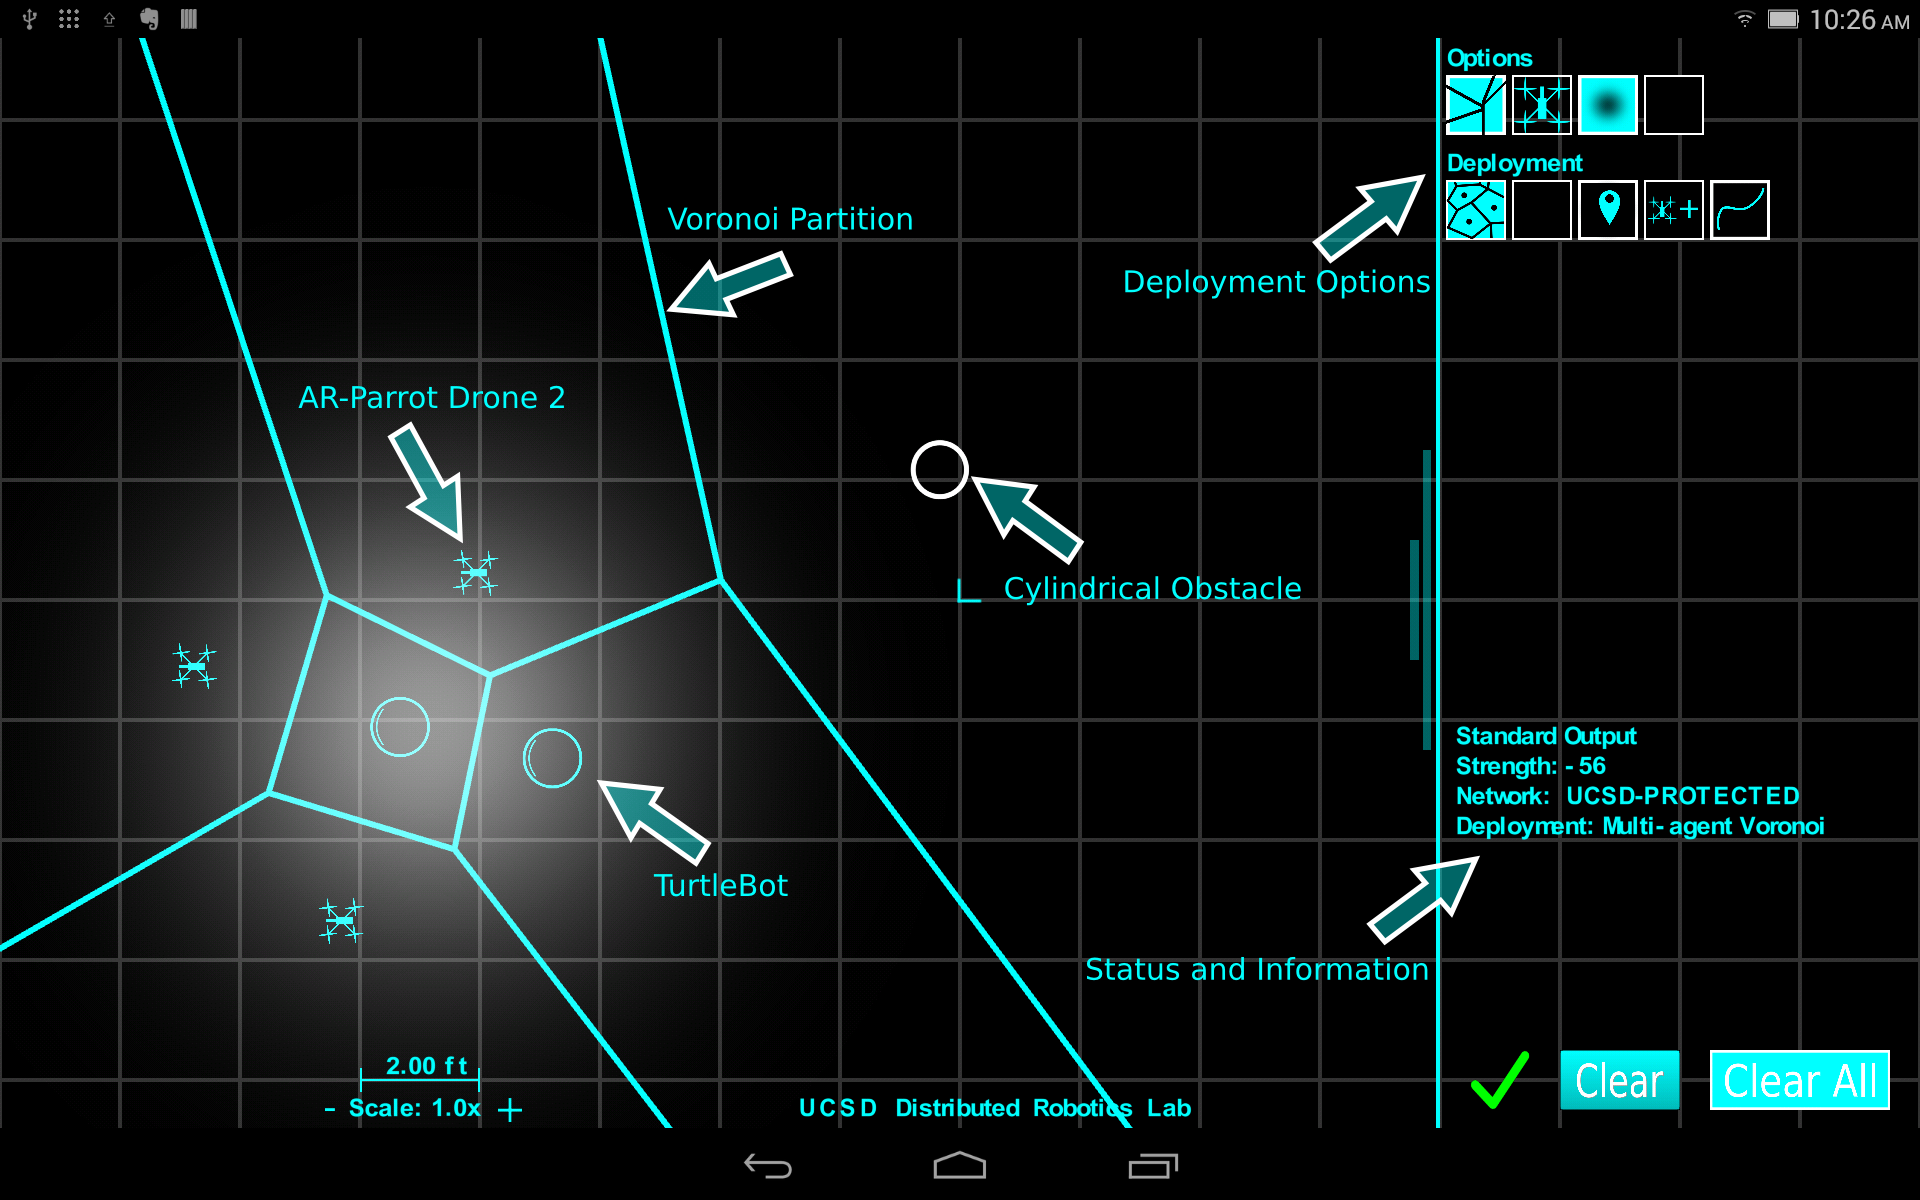
\includegraphics[width=.925\linewidth]{android_interface}}
  \end{minipage}

  \onslide<3>

  \begin{center}
    \begin{tabular}{c}
      \movie[width=.8\linewidth,showcontrols]
      {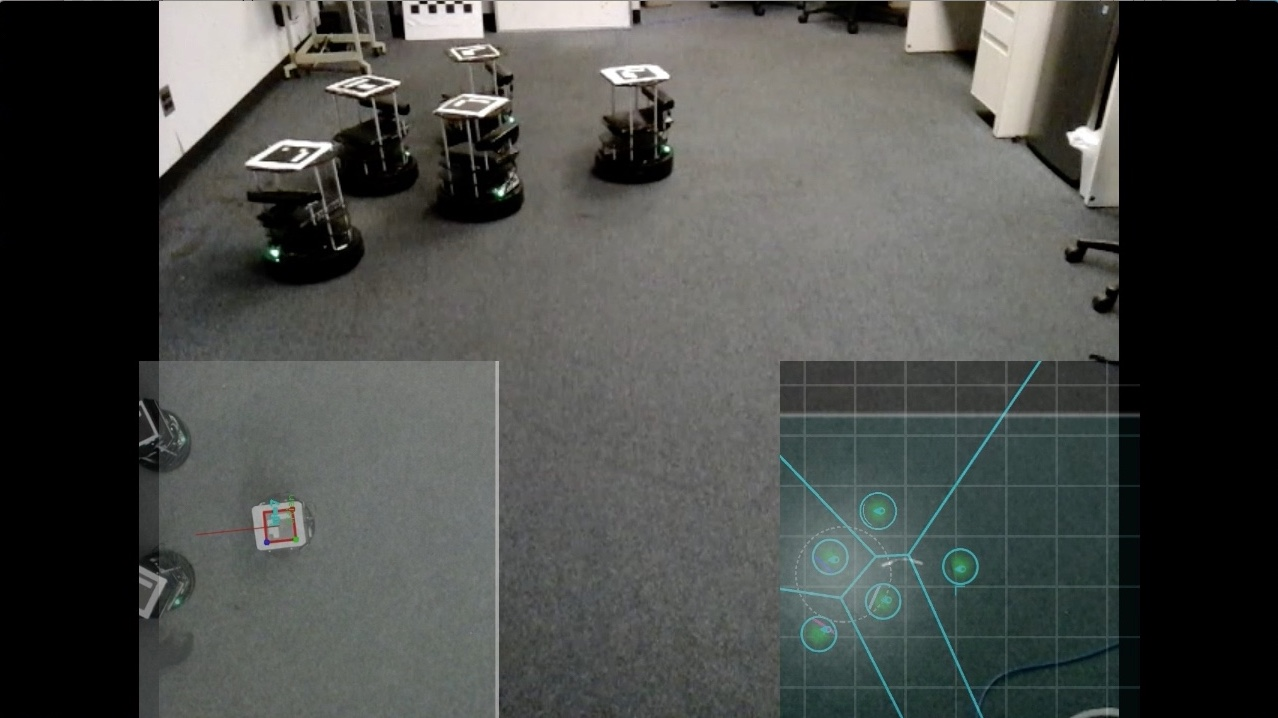
\includegraphics[width=.8\linewidth]{normal_2x}}
      {movies/gaussian_normal_moving.mov}
    \end{tabular}
  \end{center}

  \end{overprint}
  
\end{frame}
  
\end{document}
